\section{Status Update}

\begin{itemize}
	\item Clustering in the strategic model
	\item Latest system architecture
	\item Previous priorities
	\item Project steps going forward
\end{itemize}

\section{Clustering}
% \pgfkeys{
	/hexagon/.is family, /hexagon,
	default/.style = {
	},
}
\newcommand{\drawClusteringFunctionalLocation}[1][]{
	\pgfkeys{/hexagon, default, #1}

	\begin{tikzpicture}[font=\footnotesize, scale=0.5, line width=1.05]
		\draw (0,0) node[circle] {A};
	\end{tikzpicture}
}

% \drawClusteringFunctionalLocation[]

I am not sure if you remember this Brian but a while back we
talked about clustering work orders in the algorithm. I have written
it down in my notes that clustering on either \textbf{functional location}
or \textbf{platform location} was the two properties that made the most
sense.

I know that this topic was not part of the priorities in the previous memo that
I sent out to you, but I had to implement it in the code to submit the paper. I
will quickly explain the general idea with only the functional location part. I
have based the calculations on figure~\ref{fig:functional-location} which is an
image that you send Brian:

\begin{figure}[H]
	\centering
	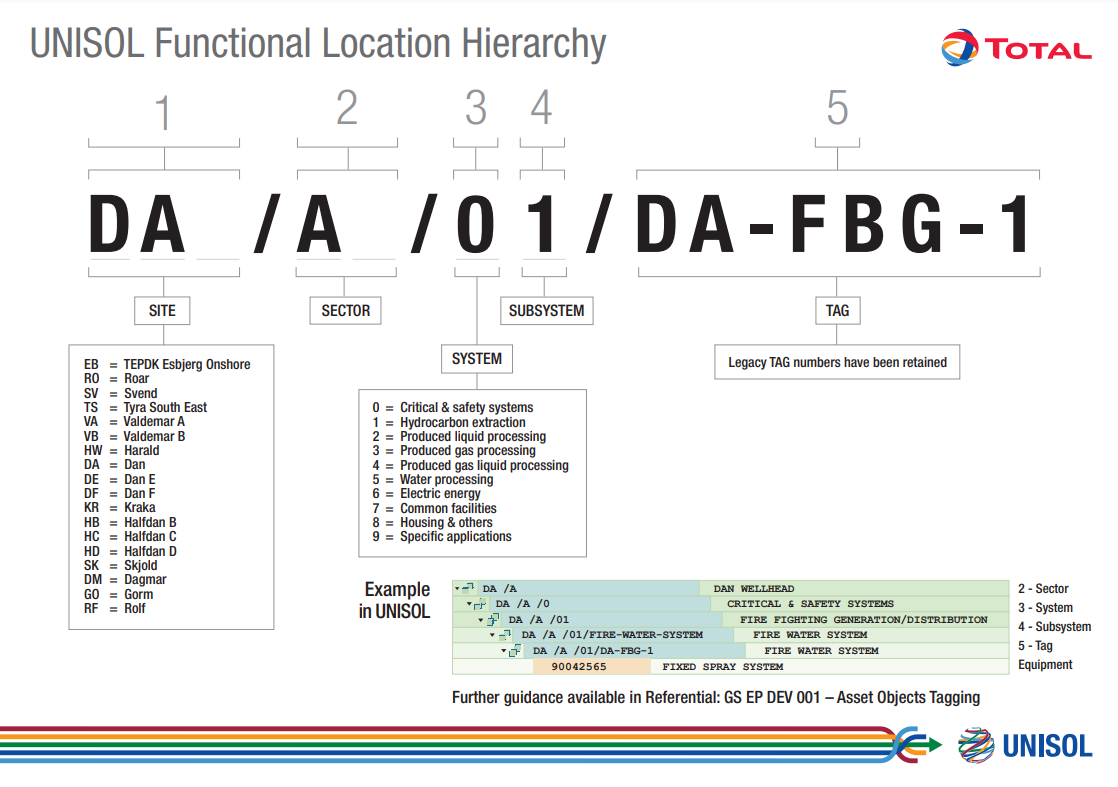
\includegraphics[width=10cm]{../../../figures/total-figures/functional_location_total.png}\label{fig:functional-location}
	\caption{Functional location hierarchy for clustering calculation}
\end{figure}

In equation~\ref{eqn:clustering} a similarity between all the work order based on their functional
location as shown below:

\newcommand{\Highlight}[2]{\colorbox{#2}{#1}}
\begin{equation}
	\begin{aligned}
		clus&tering\_value_{wo1, wo2}=  \\
		      \ \ & if \ \ SITE_{wo1}      & == & \ \  SITE_{wo2}      &\ \ \{ +20 \} \\ 
		    + \ \ & if \ \ SECTOR_{wo1}    & == & \ \  SECTOR_{wo2}    &\ \ \{ +10 \} \\ 
		    + \ \ & if \ \ SYSTEM_{wo1}    & == & \ \  SYSTEM_{wo2}    &\ \ \{ +10 \} \\ 
		    + \ \ & if \ \ SUBSYSTEM_{wo1} & == & \ \  SUBSYSTEM_{wo2} &\ \ \{ +10 \} \\ 
		    + \ \ & if \ \ TAG_{wo1}       & == & \ \  TAG_{wo2}       &\ \ \{ +50 \} \\ 
	\end{aligned}
	\label{eqn:clustering}
\end{equation}

This $clustering\_value_{wo1, wo2}$ in equation~\ref{eqn:clustering} is then calculated for all \textbf{released} work orders
for a given asset that the algorithm in initialized on. In table~\ref{tab:clustering-matrix} will now go through a small
example to show how this could look like.

\begin{table}[H]
	\centering
	\begin{tabular}{lrrrrr}
		\toprule 
		\textbf{Functional Location} & \textbf{Site} & \textbf{Sector} & \textbf{System} & \textbf{Sybsystem} & \textbf{Tag} \\
		\midrule  
		\textbf{2100000001} & DF & B & 3 & 6 & DFBA-FA-4004\\
		\textbf{2100000002} & DF & B & 3 & 6 & DFBA-FA-4004\\
		\textbf{2100000003} & DF & B & 2 & 3 & DFFA-LIT-500106\\
		\bottomrule
	\end{tabular}
	\caption{\parbox{0.6\textwidth}{Functional locations for three different example work orders}}

\end{table}

Using the data in Table~\ref{tab:clustering-matrix} we can calculate the following matrix so
similarity between the different work orders.

\begin{table}[ht]
	\centering
	\label{tab:clustering-matrix}
	\begin{tabular}{|l|c|c|c|}
		\toprule
		\textbf{Work Orders}& \textbf{2100000001}        & \textbf{2100000002}         & \textbf{2100000003} \\
		\midrule
		\textbf{2100000001} & -                          & \Highlight{100}{dtu-green}  & \Highlight{30}{dtu-yellow} \\
		\midrule
		\textbf{2100000002} & \Highlight{100}{dtu-green} & -                           & \Highlight{30}{dtu-yellow} \\
		\midrule
		\textbf{2100000003} & \Highlight{30}{dtu-yellow} & \Highlight{30}{dtu-yellow}  & - \\
		\bottomrule
	\end{tabular}
	\caption{\parbox{0.8\textwidth}{Clustering values between work orders based on functional location. Yellow values are
		calculated as: 20 + 12 = \Highlight{30}{dtu-yellow} (SITE and SECTOR), and the green values have been calculated as:
		20 + 10 + 10 + 10 + 50 = \Highlight{100}{dtu-green} (SITE, SECTOR, SYSTEM, SUBSYSTEM, and TAG)}}
\end{table}

To see where this goes into the strategic model, refer to \textbf{red} part in the model in Section~\ref{sec:strategic-model}.

\section{Latest Architecture}
I have updated the system architecture a little bit
\usetikzlibrary {positioning}
\newcommand{\drawHexagon}[6][draw=black]{
	\draw[#1, fill=#4] (#2,#3) ++(30:#6) -- ++(90:#6) -- ++(150:#6) -- ++(210:#6) -- ++(270:#6) -- ++(330:#6) -- cycle;
	\node[align=center] at (#2,#3+2) {#5};
}

\newif\ifpersistencelayer
\newif\ifatomicpointerswaplayer
\newif\ifmetaheuristicslayer
\newif\ifuserinterfacelayer
\newif\iforchestratorlayer
\newif\ifsimplifiedlayer

\pgfkeys{
	/hexagon/.is family, /hexagon,
	default/.style = {
		persistence=false,
		atomicpointerswap=false,
		metaheuristics=false,
		orchestrator=false,
		userinterface=false,
		simplified=false,
	},
	persistence/.is if=persistencelayer,
	atomicpointerswap/.is if=atomicpointerswaplayer,
	metaheuristics/.is if=metaheuristicslayer,
	orchestrator/.is if=orchestratorlayer,
	userinterface/.is if=userinterfacelayer,
	simplified/.is if=simplifiedlayer,
}
\newcommand{\drawModelSetupHexagon}[1][]{
	\pgfkeys{/hexagon, default, #1}

	\begin{tikzpicture}[font=\footnotesize, scale=0.5, line width=1.05]
	

	\ifpersistencelayer
		\drawHexagon[draw=none]{ 2                      }{ 2}{dtu-blue}{}{2}
		\drawHexagon[draw=none]{{6 - 2 * (2 - sqrt(3)) }}{ 2}{dtu-blue}{}{2}
		\drawHexagon[draw=none]{{4 - 1 * (2 - sqrt(3)) }}{-1}{dtu-blue}{Persistence}{2}
		\drawHexagon[draw=none]{{0 + 1 * (2 - sqrt(3)) }}{-1}{dtu-blue}{}{2}
		\drawHexagon[draw=none]{{8 - 3 * (2 - sqrt(3)) }}{-1}{dtu-blue}{}{2}

		\drawHexagon[draw=none]{{2 - 0 * (2 - sqrt(3)) }}{-4}{dtu-blue}{}{2}
		\drawHexagon[draw=none]{{6 - 2 * (2 - sqrt(3)) }}{-4}{dtu-blue}{}{2}

		\drawHexagon[draw=none]{{10 - 4 * (2 - sqrt(3)) }}{-4}{dtu-blue}{}{2}
		\drawHexagon[draw=none]{{-2 + 2 * (2 - sqrt(3)) }}{-4}{dtu-blue}{}{2}

		\drawHexagon[draw=none]{{12 - 5 * (2 - sqrt(3)) }}{-1}{dtu-blue}{}{2}
		\drawHexagon[draw=none]{{-4 + 3 * (2 - sqrt(3)) }}{-1}{dtu-blue}{}{2}
		% Legend for each layer
		\drawHexagon{{14.0  }}{+3.0}{dtu-blue}{}{0.75}
		\node[align=right, anchor=west] at ({15.0}, +3.75) {Persistence};
		\drawHexagon{{14.0  }}{+1.5}{dtu-white}{}{0.75}
		\node[align=right, anchor=west] at ({15.0}, +2.25) {Atomic Pointer};
		\drawHexagon{{14.0  }}{+0.0}{dtu-white}{}{0.75}
		\node[align=right, anchor=west] at ({15.0}, +0.75) {Metaheuristics};
		\drawHexagon{{14.0  }}{-1.5}{dtu-white}{}{0.75}
		\node[align=right, anchor=west] at ({15.0}, -0.75) {Orchestration};
		\drawHexagon{{14.0  }}{-3.0}{dtu-white}{}{0.75}
		\node[align=right, anchor=west] at ({15.0}, -2.25) {User interfaces};
	\fi


	\ifatomicpointerswaplayer
		\drawHexagon[]{ 2                      }{ 2}{dtu-green}{Shared\\solution\\pointer}{2}
		\drawHexagon[]{{6 - 2 * (2 - sqrt(3)) }}{ 2}{dtu-green}{Shared\\solution\\pointer}{2}
		\drawHexagon[]{{4 - 1 * (2 - sqrt(3)) }}{-1}{dtu-green}{Shared\\solution\\pointer}{2}
		\drawHexagon[]{{0 + 1 * (2 - sqrt(3)) }}{-1}{dtu-green}{Shared\\solution\\pointer}{2}
		\drawHexagon[]{{8 - 3 * (2 - sqrt(3)) }}{-1}{dtu-green}{Shared\\solution\\pointer}{2}

		\drawHexagon[]{{2 - 0 * (2 - sqrt(3)) }}{-4}{dtu-green}{Shared\\solution\\pointer}{2}
		\drawHexagon[]{{6 - 2 * (2 - sqrt(3)) }}{-4}{dtu-green}{Shared\\solution\\pointer}{2}

		\drawHexagon[]{{10 - 4 * (2 - sqrt(3)) }}{-4}{dtu-green}{Shared\\solution\\pointer}{2}
		\drawHexagon[]{{-2 + 2 * (2 - sqrt(3)) }}{-4}{dtu-green}{Shared\\solution\\pointer}{2}

		\drawHexagon[]{{12 - 5 * (2 - sqrt(3)) }}{-1}{dtu-green}{Shared\\solution\\pointer}{2}
		\drawHexagon[]{{-4 + 3 * (2 - sqrt(3)) }}{-1}{dtu-green}{Shared\\solution\\pointer}{2}
		% Legend for each layer
		\drawHexagon{{14.0  }}{+3.0}{dtu-white}{}{0.75}
		\node[align=right, anchor=west] at ({15.0}, +3.75) {Persistence};
		\drawHexagon{{14.0  }}{+1.5}{dtu-green}{}{0.75}
		\node[align=right, anchor=west] at ({15.0}, +2.25) {Atomic Pointer};
		\drawHexagon{{14.0  }}{+0.0}{dtu-white}{}{0.75}
		\node[align=right, anchor=west] at ({15.0}, +0.75) {Metaheuristics};
		\drawHexagon{{14.0  }}{-1.5}{dtu-white}{}{0.75}
		\node[align=right, anchor=west] at ({15.0}, -0.75) {Orchestration};
		\drawHexagon{{14.0  }}{-3.0}{dtu-white}{}{0.75}
		\node[align=right, anchor=west] at ({15.0}, -2.25) {User interfaces};
	\fi

	\ifsimplifiedlayer

		\node[align=right, anchor=west] at ({-5.5}, +3.75) {};
		\drawHexagon{{+2 + 0 * (2 - sqrt(3)) }}{ 2}{dtu-green}{Scheduler}{2}
		\drawHexagon{{+4 - 1 * (2 - sqrt(3)) }}{-1}{dtu-red}{Supervisor}{2}
		\drawHexagon{{+0 + 1 * (2 - sqrt(3)) }}{-1}{dtu-red}{Supervisor}{2}
		\drawHexagon{{+2 - 0 * (2 - sqrt(3)) }}{-4}{dtu-corporate-red}{Technician}{2}
		\drawHexagon{{+6 - 2 * (2 - sqrt(3)) }}{-4}{dtu-corporate-red}{Technician}{2}
		\drawHexagon{{-2 + 2 * (2 - sqrt(3)) }}{-4}{dtu-corporate-red}{Technician}{2}
		\drawHexagon{{+8 - 3 * (2 - sqrt(3)) }}{-1}{dtu-corporate-red}{Technician}{2}
		\drawHexagon{{-4 + 3 * (2 - sqrt(3)) }}{-1}{dtu-corporate-red}{Technician}{2}

		% Scheduler
		\draw[thin, fill=dtu-yellow] (2, 5) circle (0.35);
		\draw[thin, fill=dtu-purple] (2, 3) circle (0.35);
		% Supervisor 1
		\draw[thin, fill=dtu-yellow] ({+4 - 1 * (2 - sqrt(3)) }, 02) circle (0.35);
		\draw[thin, fill=dtu-purple] ({+4 - 1 * (2 - sqrt(3)) }, -0) circle (0.35);
		% Supervisor 2
		\draw[thin, fill=dtu-yellow] ({+0 + 1 * (2 - sqrt(3)) }, 02) circle (0.35);
		\draw[thin, fill=dtu-purple] ({+0 + 1 * (2 - sqrt(3)) }, -0) circle (0.35);
		% Technician 1
		\draw[thin, fill=dtu-yellow] ({+2 - 0 * (2 - sqrt(3)) }, -1) circle (0.35);
		\draw[thin, fill=dtu-purple] ({+2 - 0 * (2 - sqrt(3)) }, -3) circle (0.35);
		% Technician 2
		\draw[thin, fill=dtu-yellow] ({+6 - 2 * (2 - sqrt(3)) }, -1) circle (0.35);
		\draw[thin, fill=dtu-purple] ({+6 - 2 * (2 - sqrt(3)) }, -3) circle (0.35);
		% Technician 3
		\draw[thin, fill=dtu-yellow] ({-2 + 2 * (2 - sqrt(3)) }, -1) circle (0.35);
		\draw[thin, fill=dtu-purple] ({-2 + 2 * (2 - sqrt(3)) }, -3) circle (0.35);
		% Technician 4
		\draw[thin, fill=dtu-yellow] ({+8 - 3 * (2 - sqrt(3)) }, 02) circle (0.35);
		\draw[thin, fill=dtu-purple] ({+8 - 3 * (2 - sqrt(3)) }, -0) circle (0.35);
		% Technician 5
		\draw[thin, fill=dtu-yellow] ({-4 + 3 * (2 - sqrt(3)) }, 02) circle (0.35);
		\draw[thin, fill=dtu-purple] ({-4 + 3 * (2 - sqrt(3)) }, -0) circle (0.35);

		% Legend for each layer
		\node[align=right, anchor=west] at ({12.0}, +3.75) {Atomic Pointer};
		\draw[fill=dtu-purple] (11.0,  +3.75) circle (0.5);

		\node[align=right, anchor=west] at ({12.0}, +2.25) {Scheduler Metaheuristic};
		\drawHexagon{{11.0  }}{+1.75}{dtu-green}{}{0.5}
		\node[align=right, anchor=west] at ({12.0}, +0.75) {Supervisor Metaheuristic};
		\drawHexagon{{11.0  }}{+0.25}{dtu-red}{}{0.5}
		\node[align=right, anchor=west] at ({12.0}, -0.75) {Technician Metaheuristic};
		\drawHexagon{{11.0  }}{-1.25}{dtu-corporate-red}{}{0.5}
		\node[align=right, anchor=west] at ({12.0}, -2.25) {User interfaces (Message Passing)};
		\draw[fill=dtu-yellow] (11.0, -2.25) circle (0.5);
	\fi

	\ifmetaheuristicslayer
		\drawHexagon{ 2                      }{ 2}{dtu-blue}{Strategic}{2}
		\drawHexagon{{6 - 2 * (2 - sqrt(3)) }}{ 2}{dtu-green}{Tactical}{2}
		\drawHexagon{{4 - 1 * (2 - sqrt(3)) }}{-1}{dtu-red}{Supervisor}{2}
		\drawHexagon{{0 + 1 * (2 - sqrt(3)) }}{-1}{dtu-red}{Supervisor}{2}
		\drawHexagon{{8 - 3 * (2 - sqrt(3)) }}{-1}{dtu-red}{Supervisor}{2}

		\drawHexagon{{2 - 0 * (2 - sqrt(3)) }}{-4}{dtu-corporate-red}{Technician}{2}
		\drawHexagon{{6 - 2 * (2 - sqrt(3)) }}{-4}{dtu-corporate-red}{Technician}{2}

		\drawHexagon{{10 - 4 * (2 - sqrt(3)) }}{-4}{dtu-corporate-red}{Technician}{2}
		\drawHexagon{{-2 + 2 * (2 - sqrt(3)) }}{-4}{dtu-corporate-red}{Technician}{2}

		\drawHexagon{{12 - 5 * (2 - sqrt(3)) }}{-1}{dtu-corporate-red}{Technician}{2}
		\drawHexagon{{-4 + 3 * (2 - sqrt(3)) }}{-1}{dtu-corporate-red}{Technician}{2}

		% Legend for each layer
		\drawHexagon{{14.0  }}{+3.0}{dtu-white}{}{0.75}
		\node[align=right, anchor=west] at ({15.0}, +3.75) {Persistence};
		\drawHexagon{{14.0  }}{+1.5}{dtu-white}{}{0.75}
		\node[align=right, anchor=west] at ({15.0}, +2.25) {Atomic Pointer};
		\drawHexagon{{14.0  }}{+0.0}{dtu-corporate-red}{}{0.75}
		\node[align=right, anchor=west] at ({15.0}, +0.75) {Metaheuristics};
		\drawHexagon{{14.0  }}{-1.5}{dtu-white}{}{0.75}
		\node[align=right, anchor=west] at ({15.0}, -0.75) {Orchestration};
		\drawHexagon{{14.0  }}{-3.0}{dtu-white}{}{0.75}
		\node[align=right, anchor=west] at ({15.0}, -2.25) {User interfaces};
	\fi

	\iforchestratorlayer
		\drawHexagon{ 2                      }{ 2}{dtu-orange}{}{2}
		\drawHexagon{{6 - 2 * (2 - sqrt(3)) }}{ 2}{dtu-orange}{}{2}
		\drawHexagon{{4 - 1 * (2 - sqrt(3)) }}{-1}{dtu-orange}{Orche-\\strator}{2}
		\drawHexagon{{0 + 1 * (2 - sqrt(3)) }}{-1}{dtu-orange}{}{2}
		\drawHexagon{{8 - 3 * (2 - sqrt(3)) }}{-1}{dtu-orange}{}{2}

		\drawHexagon{{2 - 0 * (2 - sqrt(3)) }}{-4}{dtu-orange}{}{2}
		\drawHexagon{{6 - 2 * (2 - sqrt(3)) }}{-4}{dtu-orange}{}{2}

		\drawHexagon{{10 - 4 * (2 - sqrt(3)) }}{-4}{dtu-orange}{}{2}
		\drawHexagon{{-2 + 2 * (2 - sqrt(3)) }}{-4}{dtu-orange}{}{2}

		\drawHexagon{{12 - 5 * (2 - sqrt(3)) }}{-1}{dtu-orange}{}{2}
		\drawHexagon{{-4 + 3 * (2 - sqrt(3)) }}{-1}{dtu-orange}{}{2}
		% Legend for each layer
		\drawHexagon{{14.0  }}{+3.0}{dtu-white}{}{0.75}
		\node[align=right, anchor=west] at ({15.0}, +3.75) {Persistence};
		\drawHexagon{{14.0  }}{+1.5}{dtu-white}{}{0.75}
		\node[align=right, anchor=west] at ({15.0}, +2.25) {Atomic Pointer};
		\drawHexagon{{14.0  }}{+0.0}{dtu-white}{}{0.75}
		\node[align=right, anchor=west] at ({15.0}, +0.75) {Metaheuristics};
		\drawHexagon{{14.0  }}{-1.5}{dtu-orange}{}{0.75}
		\node[align=right, anchor=west] at ({15.0}, -0.75) {Orchestration};
		\drawHexagon{{14.0  }}{-3.0}{dtu-white}{}{0.75}
		\node[align=right, anchor=west] at ({15.0}, -2.25) {User interfaces};
	\fi

	
	\ifuserinterfacelayer
		\drawHexagon{ 2                      }{ 2}{dtu-yellow}{UI}{2}
		\drawHexagon{{6 - 2 * (2 - sqrt(3)) }}{ 2}{dtu-yellow}{UI}{2}
		\drawHexagon{{4 - 1 * (2 - sqrt(3)) }}{-1}{dtu-yellow}{UI}{2}
		\drawHexagon{{0 + 1 * (2 - sqrt(3)) }}{-1}{dtu-yellow}{UI}{2}
		\drawHexagon{{8 - 3 * (2 - sqrt(3)) }}{-1}{dtu-yellow}{UI}{2}

		\drawHexagon{{2 - 0 * (2 - sqrt(3)) }}{-4}{dtu-yellow}{UI}{2}
		\drawHexagon{{6 - 2 * (2 - sqrt(3)) }}{-4}{dtu-yellow}{UI}{2}

		\drawHexagon{{10 - 4 * (2 - sqrt(3)) }}{-4}{dtu-yellow}{UI}{2}
		\drawHexagon{{-2 + 2 * (2 - sqrt(3)) }}{-4}{dtu-yellow}{UI}{2}

		\drawHexagon{{12 - 5 * (2 - sqrt(3)) }}{-1}{dtu-yellow}{UI}{2}
		\drawHexagon{{-4 + 3 * (2 - sqrt(3)) }}{-1}{dtu-yellow}{UI}{2}
		% Legend for each layer
		\drawHexagon{{14.0  }}{+3.0}{dtu-white}{}{0.75}
		\node[align=right, anchor=west] at ({15.0}, +3.75) {Persistence};
		\drawHexagon{{14.0  }}{+1.5}{dtu-white}{}{0.75}
		\node[align=right, anchor=west] at ({15.0}, +2.25) {Atomic Pointer};
		\drawHexagon{{14.0  }}{+0.0}{dtu-white}{}{0.75}
		\node[align=right, anchor=west] at ({15.0}, +0.75) {Metaheuristics};
		\drawHexagon{{14.0  }}{-1.5}{dtu-white}{}{0.75}
		\node[align=right, anchor=west] at ({15.0}, -0.75) {Orchestration};
		\drawHexagon{{14.0  }}{-3.0}{dtu-yellow}{}{0.75}
		\node[align=right, anchor=west] at ({15.0}, -2.25) {User interfaces};
	\fi
	
	\end{tikzpicture}
}

\begin{figure}[H]
	\centering
    \drawModelSetupHexagon[simplifiedtechnicallanguage=true]
	\caption{\parbox{0.8\textwidth}{Every algorithm has its own user interface. This means that there will be a view into the system that is 
		unique for each kind of stakeholder.}
	}\label{fig:hexagon:simplified}
\end{figure}

\section{Priorities}
Currently my priorities are:
\begin{itemize} 
	\item Backend: Make the tactical algorithm dynamic and functioning respect constraints 
	\item Frontend: Let you manually upload resources
	\item Frontend: Let you see live updating of the currect resource profile of the schedule 
		that the algorithm is generating.
\end{itemize}

So questions for you if you disagree with the priorities:
\begin{itemize}
	\item \colorbox{yellow}{\textbf{What aspects of the program does each of you think should be prioritized now?}}
	\item \colorbox{yellow}{\textbf{I believe that making this program work without any involvement of a offshore}}	\\
    	\colorbox{yellow}{\textbf{supervisor (the person responsible for assigning names to the technicians) }} \\
		\colorbox{yellow}{\textbf{will be very difficult. Do you aggee or disagree?}}
\end{itemize} 
